\documentclass[11pt, openright]{book}

    % Cover Variables
    \newcommand{\ctoptitle}{RAPPORT DE SYNTHÈSE}
    \newcommand{\ctitle}{STAGE OPERATIONNEL}
    \newcommand{\cautor}{Lucas Lescure}
    \newcommand{\cdate}{27.05.2024/21.06.2024}
    \newcommand{\sectittle}{Capteur à fibre optique}
    \newcommand{\sectoptittle}{pour les environment extrèmes}


    % Header Variables
        \newcommand{\headRE}{Stage opérationnel}
        \newcommand{\headLE}{\emph{\rightmark}}
        \newcommand{\footRE}{Lucas Lescure $-$ \cdate}
        \newcommand{\footLE}{\emph{\thepage}}

    % TOC Variables
        \newcommand{\toctitle}{Table des Matières}
        
        \newcommand{\tocchapter}{Chapter}
        \newcommand{\toccount}{2}
  
    % Chapter Variables
        \newcommand{\chvar}{Chapter -}

\usepackage[a4paper, total={16cm, 22.125cm}]{geometry}

% Page Style
\usepackage[]{environ}
% Cover Page 
\usepackage{tikz}
\makeatletter
\def\parsecomma#1,#2\endparsecomma{\def\page@x{#1}\def\page@y{#2}}
\tikzdeclarecoordinatesystem{page}{
    \parsecomma#1\endparsecomma
    \pgfpointanchor{current page}{north east}
    % Save the upper right corner
    \pgf@xc=\pgf@x%
    \pgf@yc=\pgf@y%
    % save the lower left corner
    \pgfpointanchor{current page}{south west}
    \pgf@xb=\pgf@x%
    \pgf@yb=\pgf@y%
    % Transform to the correct placement
    \pgfmathparse{(\pgf@xc-\pgf@xb)/2.*\page@x+(\pgf@xc+\pgf@xb)/2.}
    \expandafter\pgf@x\expandafter=\pgfmathresult pt
    \pgfmathparse{(\pgf@yc-\pgf@yb)/2.*\page@y+(\pgf@yc+\pgf@yb)/2.}
    \expandafter\pgf@y\expandafter=\pgfmathresult pt
}
\makeatother


% Object formatting
\usepackage[12pt]{moresize}
\usepackage[]{anyfontsize}
\usepackage{titlesec}
\usepackage{import}
\usepackage{floatrow}
\usepackage{enumitem}
\usepackage{changepage}
\usepackage[normalem]{ulem}
\usepackage{array}
\newcommand{\ul}[1]{\underline{#1}}

\usepackage[]{chngcntr}
\usepackage{ifthen}
\ifthenelse{\figcountdepth > 1}
  {\counterwithin{figure}{section}\counterwithin{table}{section}}
  {}

\usepackage[format=plain, labelfont=it, textfont=it]{caption}
\makeatletter
\def\@makecaption#1#2{%
    \vskip\abovecaptionskip
    \sbox\@tempboxa{\textit{#1.} #2}

       
   

    \ifdim \wd\@tempboxa >\hsize
        #1. #2\par
    \else
        \global \@minipagefalse
        \hb@xt@\hsize{\hfil\box\@tempboxa\hfil}
    \fi
    \vskip\belowcaptionskip}
\makeatother

\DeclareCaptionFormat{underline}{\uline{#1#2#3}\par}

% Sections
\titleformat{\section}{\fontsize{16}{19.2}\bfseries}{\thesection.}{0.25em}{}
\titleformat{\subsection}{\fontsize{14}{16.8}\bfseries}{\tab\thesubsection.}{0.25em}{}
\titleformat{\subsubsection}{\fontsize{10}{12}}{\uline{\thesubsubsection)\enspace}}{0em}{\uline}





% Geometry

% Typewritting

\setlength{\parskip}{1em}
\setlength{\parindent}{0em}


\newenvironment{items}[3][0pt]
{\def\closesep{#3}
    \vspace{#2}
    \begin{itemize}
        \setlength{\itemsep}{#1}
        \setlength{\topsep}{0pt}
        \setlength{\partopsep}{0pt}}
        {\end{itemize}
    \vspace{\closesep}}

\newenvironment{enum}[3][0pt]
{\defclosesep{#3}
    \vspace{#2}
    \begin{enumerate}
        \setlength{\itemsep}{#1}
        \setlength{\topsep}{0pt}
        \setlength{\partopsep}{0pt}}
        {\end{enumerate}
    \vspace{\closesep}}

\newenvironment{eq}[2]
{\def\closesep{#2}
    \vspace{#1}
    \begin{align*}}
        {\end{align*}
    \vspace{\closesep}}

\newenvironment{lfeq}[2]
{\def\closesep{#2}
    \vspace{#1}
    \begin{flalign*}}
        {\end{flalign*}
    \vspace{\closesep}}
% List Formatting


\NewEnviron{dent}[1]{
    \vspace{-10pt}
    \begin{adjustwidth}{7mm}{}
        \uline{#1}\hspace{2mm}
        \BODY
    \end{adjustwidth}
    \vspace{-10pt}
}


\usepackage[framemethod=tikz]{mdframed}
\newcounter{count_theorem}[section]\setcounter{count_theorem}{0}
\newcommand{\thetheorem}{\arabic{count_theorem}}

\newcounter{count_exercise}[section]\setcounter{count_exercise}{0}
\newcommand{\theexercise}{\arabic{count_exercise}}


\newenvironment{theorem}[1][]{
    \refstepcounter{count_theorem}
    \mdfsetup{
        linecolor=red!30,
        innerbottommargin=10pt,
        linewidth=2pt,
        topline=false,
        bottomline=false,
        rightline=false,
        shadow=true,
        shadowsize=4.5pt,
        frametitlerule=false,
        apptotikzsetting={
                \tikzset{
                    mdfbackground/.append style={
                            left color=red!8,right color=red!3
                        }
                }
            }
    }
    \begin{mdframed}[]\relax
        \ifstrempty{#1}
        {\textbf{Theorem~\thetheorem.} }
        {\textbf{Theorem~\thetheorem.~#1} }
        }
        {\end{mdframed}\vspace{-10pt}
}

\newenvironment{note}{
    \mdfsetup{innertopmargin=5pt,
        linecolor=gray!30,
        linewidth=2pt,
        topline=false,
        bottomline=false,
        rightline=false,
        frametitleaboveskip=0pt,
        shadow=false,
        shadowsize=4pt,
        frametitlerule=false,
        apptotikzsetting={
                \tikzset{
                    mdfbackground/.append style={
                            left color=gray!8,right color=gray!3
                        }
                }
            }
    }
    \begin{mdframed}[]\relax
        \textbf{Note. }
        }
        {\end{mdframed}\vspace{-10pt}
}

\newenvironment{example}{
    \mdfsetup{innertopmargin=5pt,
        linecolor=green!30,
        linewidth=2pt,
        topline=false,
        bottomline=false,
        rightline=false,
        frametitleaboveskip=0pt,
        shadow=false,
        shadowsize=4pt,
        frametitlerule=false,
        apptotikzsetting={
                \tikzset{
                    mdfbackground/.append style={
                            left color=green!7,right color=green!2
                        },
                    mdfframetitlebackground/.append style={
                            left color=green!7,right color=green!2
                        }
                }
            }
    }
    \begin{mdframed}[]\relax
        \textbf{Example. }
        }
        {\end{mdframed}\vspace{-10pt}
}


\usetikzlibrary{calc,arrows}

\tikzset{
    excursus arrow/.style={%
            line width=2pt,
            draw=gray!40,
            rounded corners=2ex,
        },
    excursus head/.style={
            fill=white,
            font=\bfseries\sffamily,
            text=gray!80,
            anchor=base west,
        },
    excursus line/.style={%
            line width=2pt,
            draw=gray!40,
            rounded corners=2ex,
        }
}

\newenvironment{exercise}[1][]{%
    \refstepcounter{count_exercise}
    \mdfsetup{
        singleextra={
                \path let \p1=(P), \p2=(O) in (\x2,\y1) coordinate (Q);
                \path let \p1=(Q), \p2=(O) in (\x1,{(\y1-\y2)/2}) coordinate (M);
                \path [excursus line] ($(O)+(5em,0ex)$) -| (M) |- ($(Q)+(20em,0ex)$);
                \node [excursus head] at ($(Q)+(2.5em,-0.75pt)$) {\ifstrempty{#1}{Exercise \theexercise}{Exercise \theexercise:~#1}};},
        firstextra={
                \path let \p1=(P), \p2=(O) in (\x2,\y1) coordinate (Q);
                \path [excursus arrow,-to] (O) |- ($(Q)+(12em,0ex)$) .. controls +(0:16em) and +(185:6em) .. ++(23em,2ex);},
        middlelinewidth=2.5em,middlelinecolor=white,
        hidealllines=true,topline=true,
        innertopmargin=0.5ex,
        innerbottommargin=2.5ex,
        innerrightmargin=2pt,
        innerleftmargin=2ex,
        skipabove=0.87\baselineskip,
        skipbelow=0.62\baselineskip,
    }
    \begin{mdframed}[]\relax}
        {\end{mdframed}\vspace{-10pt}
}

% Functions and Data Plotting
\usepackage{subfig,wrapfig,adjustbox,multirow}


% Plotting Style
\usepackage{graphicx,pgfplots}
\usetikzlibrary{arrows}
\usetikzlibrary {patterns,patterns.meta}
\usepgfplotslibrary{fillbetween}
\pgfplotsset{compat=1.18}

\usepgfplotslibrary{units}
% Logarithmic Scale
\pgfplotsset{
    log x ticks with fixed point/.style={
            xticklabel={
                    \pgfkeys{/pgf/fpu=true}
                    \pgfmathparse{exp(\tick)}%
                    \pgfmathprintnumber[fixed relative, precision=3]{\pgfmathresult}
                    \pgfkeys{/pgf/fpu=false}
                }
        }
}


% Mathematics

% Formatting
\usepackage{amsmath}
\usepackage{esvect}
\usepackage{amsfonts}
\usepackage{tasks,environ}
\usepackage{xargs}
\usepackage{esint}
\usepackage[]{listings}


\usepackage[english]{babel}
\usepackage{amsthm}
%\newtheorem{theorem}{Theorem}
%\newtheorem{proof}{Proof}



%Custom Shortcuts
\newcommand{\eqi}{\Leftrightarrow}
\newcommand{\lr}[1]{\left( #1 \right)}
\newcommand{\limit}[1]{\displaystyle{\lim_{#1}}}
\newcommand{\tab}{\hspace*{7mm}}
\newcommand{\ds}[1]{\displaystyle{#1}}
\newcommand{\floor}[1]{\lfloor #1 \rfloor}
\newcommand{\R}{\mathbb{R}}
\newcommand{\N}{\mathbb{N}}
\newcommand{\Z}{\mathbb{Z}}
\newcommand{\C}{\mathbb{C}}
\newcommand{\K}{\mathbb{K}}
\newcommand{\F}{\mathcal{F}}
\newcommand{\M}{\mathcal{M}}
\renewcommand{\l}{\lambda}
\newcommand{\seg}[1]{\overline{\rm {#1}}}
\newcommand{\Int}{\int\limits}
\newcommand{\ex}{\tab \uline{Example :}\hspace{0.2cm} }
\newcommand{\vard}{\partial}
\newcommand{\Q}{\mathcal{Q}}
\newcommand{\Vect}{\operatorname{Vect}}
\newcommand{\rg}{\operatorname{rg}}
\renewcommand{\dim}{\operatorname{dim}}
\renewcommand{\Re}{\operatorname{Re}}
\renewcommand{\Im}{\operatorname{Im}}
\renewcommand{\P}{\mathcal{P}}
\newcommand{\blr}[1]{\left\{#1\right\}}
\newcommand{\linecenter}[1]{\par\vspace{2mm} \centerline{#1}\par\vspace{-2mm}}
\newcommand{\dd}{\textrm{d}}
\newcommand{\supp}{\operatorname{Supp}}
\renewcommand{\vec}{\overrightarrow}
\renewcommand{\epsilon}{\varepsilon}

% Matrix Configurations

\makeatletter
\renewcommand*\env@matrix[1][*\c@MaxMatrixCols c]{%
    \hskip -\arraycolsep
    \let\@ifnextchar\new@ifnextchar
    \array{#1}}
\makeatother


% Colors
\usepackage{xcolor}
\newcommand{\blu}{\color{blue}}
\newcommand{\Red}{\color{red}}
\newcommand{\blac}{\color{black}}

\newcommand{\red}[1]{\textcolor{red}{#1}}

\usepackage{xcolor,xspace}
\usepackage{breqn}


% Headings  
\usepackage[Glenn]{fncychap}
\ChNumVar{\fontsize{40}{42}}
\ChTitleVar{\Large\sc}
\ChNameVar{\Large\sc}
\setlength\headheight{14.5pt}
\renewcommand\FmN[1]{\chvar}



\usepackage{fancyhdr}
\usepackage{ragged2e}

% Header & Footers
\renewcommand{\chaptermark}[1]{\markboth{#1}{#1}}
\renewcommand{\sectionmark}[1]{
    \markright{ #1}
}
\pagestyle{fancy}
\fancyhf{}
\fancyhead[LE,RO]{\headLE}
\fancyhead[RE,LO]{\headRE}
\fancyfoot[LE,RO]{\footLE}
\fancyfoot[RE,LO]{\footRE}
\renewcommand{\headrulewidth}{0.5pt}
\fancyheadoffset{1cm}

\fancypagestyle{plain}{%
    \fancyhf{} % clear all header and footer fields
    \fancyfoot[LE, RO]{\footLE}
    \renewcommand{\headrulewidth}{0pt}
    \renewcommand{\footrulewidth}{0pt}}


\fancypagestyle{nohead}{%
    \fancyhf{} % clear all header 
    \fancyfoot[LE, RO]{\footLE}
    \fancyfoot[LO, RE]{\footRE}}

    \fancypagestyle{head}{%
    \fancyhf{} % clear all header 
    \fancyhead[LE,RO]{\headLE}
\fancyhead[RE,LO]{\headRE}
\renewcommand{\headrulewidth}{0.5pt}
\fancyheadoffset{1cm}
    }


\fancypagestyle{bib}{%
    \fancyhf{} % clear all header and footer fields
    \fancyhead[CE, CO]{}
    \fancyfoot[LE, RO]{\footLE}
    \fancyfoot[LO, RE]{Bibliographie}}

% Table of Contents

\renewcommand*\thechapter{\arabic{chapter}} %Usually Roman
\renewcommand*\thesection{\arabic{section}}
\renewcommand*\thesubsubsection{\thesubsection.\alph{subsubsection}}
\makeatletter
\@removefromreset{section}{chapter}
\makeatother


% Table of Contents

\usepackage{titletoc}
\usepackage{ erewhon,cabin}
\usepackage[linktoc=all]{hyperref}
\renewcommand*\contentsname{\centerline{\toctitle}}

\setcounter{secnumdepth}{3}
\setcounter{tocdepth}{\toccount}

\usepackage[subfigure]{tocloft}
\setlength\cftparskip{0pt}

\usepackage{etoolbox}
\makeatletter
\pretocmd{\chapter}{\addtocontents{toc}{\protect\addvspace{5\p@}}}{}{}
\pretocmd{\section}{\addtocontents{toc}{\protect\addvspace{-10\p@}}}{}{}
\pretocmd{\subsection}{\addtocontents{toc}{\protect\addvspace{1\p@}}}{}{}
\makeatother


% Chapter Style
\titlecontents{chapter}
[11em]
{\bigskip}
{\bfseries\textsc\tocchapter~\textsc\thecontentslabel : \textsc}
{\hspace*{-5.5em}\textbf}
{\titlerule*[1pc]{ }}[\smallskip]

% Section Style
\titlecontents{section}
[0em] % i
{\bigskip\bfseries}
{\fontsize{11}{13.2}\bfseries\uline{\thecontentslabel.\enspace}\uline}
{\hspace*{-4em}\textbf}
{\hspace{0.5pt}\uline{\hspace*{\fill}}\contentspage}

% Subsection Style
\titlecontents{subsection}
[2em] % i
{\smallskip\bfseries}
{\fontsize{10}{12}\bfseries\thecontentslabel.\enspace}
{\hspace*{-4em}}
{\titlerule*[0.5pc]{.}\contentspage}

% Subsubsection Style
\titlecontents{subsubsection}
[4em] % i
{\smallskip}
{\fontsize{10}{12}\thecontentslabel)\enspace}
{\hspace*{-4em}}
{\titlerule*[0.5pc]{.}\contentspage}










    % figure support
    \usepackage{import}
    \usepackage{xifthen}
    \pdfminorversion=7
    \usepackage{pdfpages}
    \usepackage{transparent}
    \newcommand{\incfig}[1]{%
            \def\svgwidth{\columnwidth}
            \import{./figures/}{#1.pdf_tex}
    }

    \pdfsuppresswarningpagegroup=1


\begin{document}
% Spacing
% Section Spacing
\titlespacing\section{0pt}{3pt plus 2pt minus 2pt}{6pt plus 2pt minus 1pt}
\titlespacing\subsection{0pt}{0pt plus 1pt minus 1pt}{0pt plus 3pt minus 1pt}
\titlespacing\subsubsection{0pt}{0pt plus 0pt minus 0pt}{0pt plus 2pt minus 0pt}

\usetikzlibrary{shadows}

\newgeometry{left=2.5cm, width=16cm, bottom=2.5cm, top=2.5cm}






% Cover
% Cover
\definecolor{ccolor1}{RGB}{236,145,143}
\definecolor{ccolor2}{RGB}{131,168,192}
\definecolor{ccolor3}{RGB}{182,227,150}
\definecolor{ccolor4}{RGB}{171,206,145}

\usetikzlibrary{fadings}

\begin{titlepage}
    \newgeometry{top=1cm, width=21cm, bottom=1cm}

    \begin{tikzpicture}[remember picture,overlay,every node/.style={anchor=center}]

        \coordinate (Center) at (page cs: 0,-0.5);
        %F4E Logo
        \begin{scope}[scale = 1.5]
            \foreach \angle in {0,30,...,330} {
                    \filldraw[orange!50!yellow,line width=0.01pt,shift=(Center)] (\angle:3.8637) -- (\angle+30:3.8637) -- (0,0) -- (\angle:3.8637);
                    \draw[white, line width = 7pt,shift=(Center)] (\angle:2cm) arc (\angle-60:\angle:2cm);
                    \draw[white, line width = 7pt,shift=(Center)] (\angle+30:2cm) arc (\angle+90:\angle+30:2cm);
                }
            % Outer delimiter
            \foreach \angle in {15,45,...,345} {
                    \filldraw[white, line width = 7pt,shift=(Center)] (\angle:3.8637cm) arc (\angle-15:\angle+45:2cm) arc (\angle+15:\angle-15:2cm) arc (\angle+45:\angle+15:2cm);
                }
            % Inner delimiter
            \foreach \angle in {15,45,...,345} {
                    \filldraw[white, line width = 7pt,shift=(Center)] (\angle:1.0353cm) arc (\angle-75:\angle-45:2cm) arc (\angle+75:\angle+105:2cm) -- (0,0) -- (\angle:1.0353cm);
                }
            % Stars
            \foreach \angle in {0,30,...,330} {
                    \fill[orange!50!yellow,shift=(Center)] (\angle:1.03527cm) -- ++ (231:0.175) -- ++ (33:0.35) -- ++ (177:0.35) -- ++ (321:0.35) -- ++ (105:0.35) -- ++ (249:0.35) -- ++ (33:0.35);
                }
        \end{scope}

        \node[opacity =0.07, inner sep=0pt, anchor=east] at (current page.east){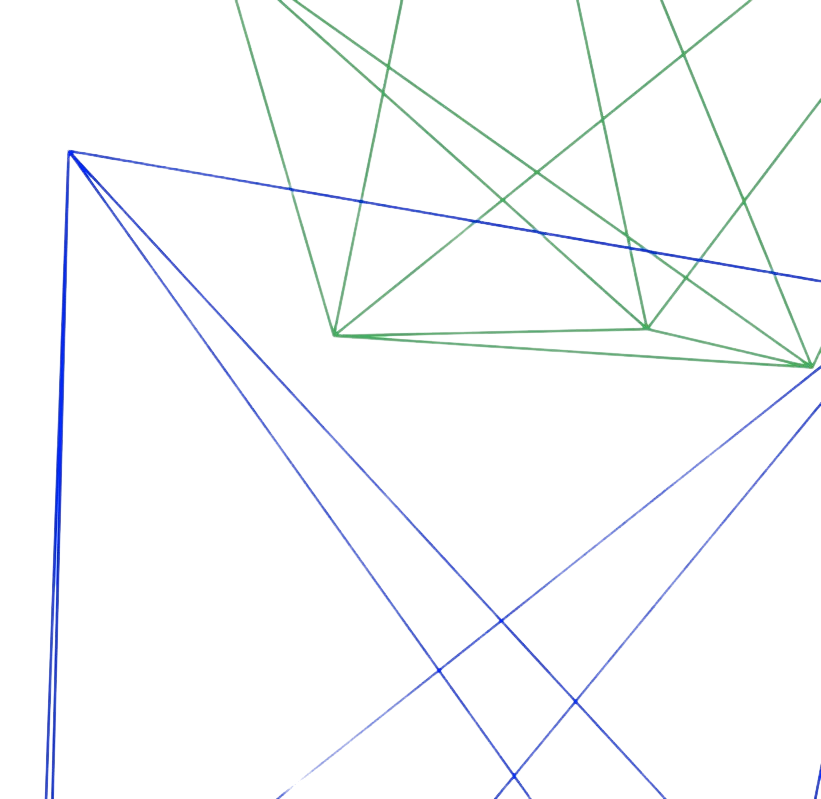
\includegraphics[width=0.5\paperwidth,height=\paperheight]{/root/.config/latex-utils/logos/invert1.png}};

        \node[opacity=0.07,inner sep=0pt, anchor=north west] at (current page.north west){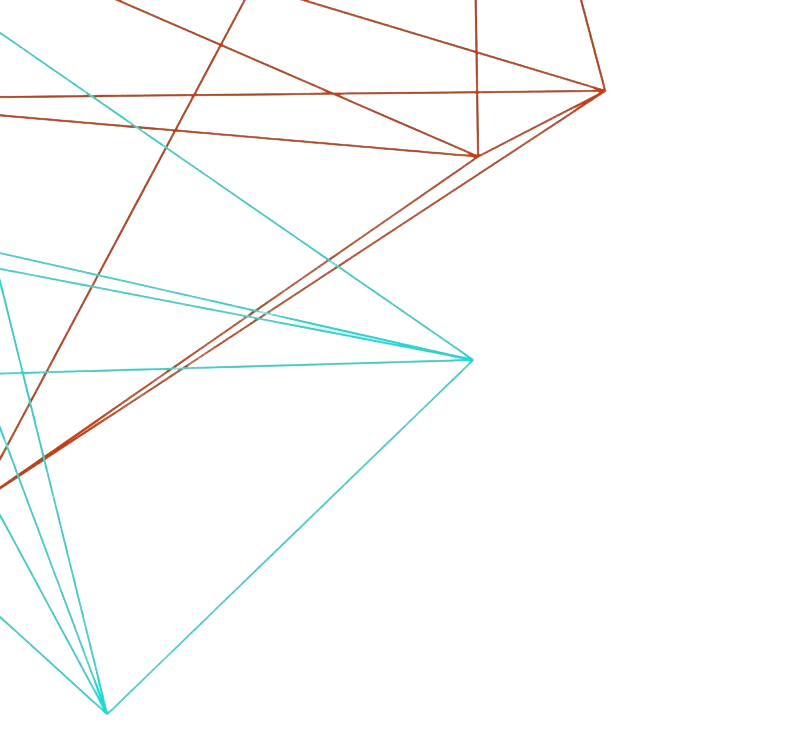
\includegraphics[width=0.5\paperwidth,height=0.5\paperheight]{/root/.config/latex-utils/logos/invert3.png}};




        \node at (page cs:0,0.345) {\Large\textsc{High School Observation and Learning Internship}};
        \node at (page cs:0,0.875) {\Large\bfseries\textsc{Observation Internship}};
        \node at (page cs:0,0.925) {\LARGE\bfseries\textsc{Lycée Français de Barcelone}};

        \node at (page cs:0.5,0) {\Large\textsc{Cyril Lescure - Pedagogical Tutor}};








        %\node[opacity=0.15, inner sep=0pt, anchor=south west] at (current page.south west){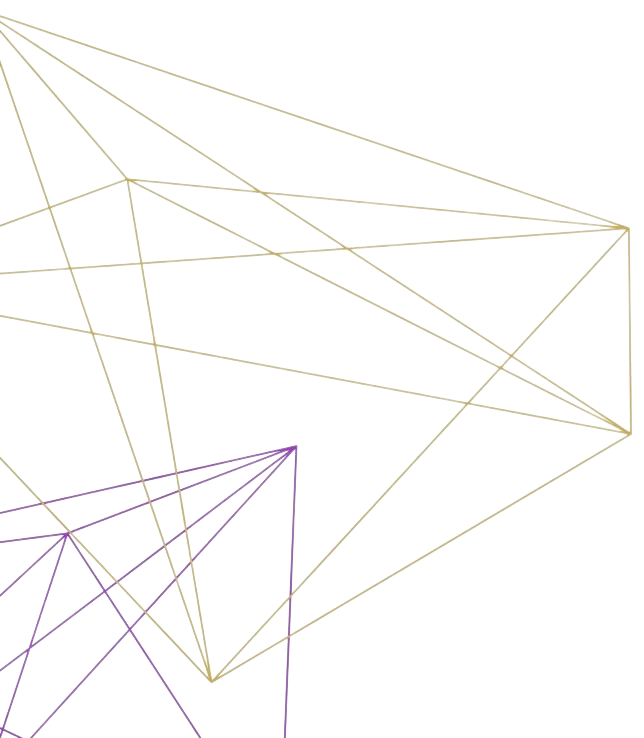
\includegraphics[width=0.5\paperwidth,height=0.5\paperheight]{/root/.config/latex-utils/logos/invert2.png}};

        \node at (page cs:0,0.5) {\fontsize{28}{28.8}\textbf{\ctoptitle}};
        \node at (page cs:0,0.425) {\fontsize{28}{28.8}\textbf{\ctitle}};
        \draw (page cs:0.5,0.375) -- (page cs:-0.5,0.375);
        \node at (page cs:0,0.245) {\LARGE\textsc{\cautor}};
        \node at (page cs:0,0.310) {\Large\textsc{03.06.2019 - 07.06.2019}};


    \end{tikzpicture}
\end{titlepage}


\newgeometry{width=18.625cm, bottom=2cm, top=2cm}

\tikz[remember picture, overlay] \node[opacity=0.3,inner sep=0pt, anchor=north east] at (current page.north east){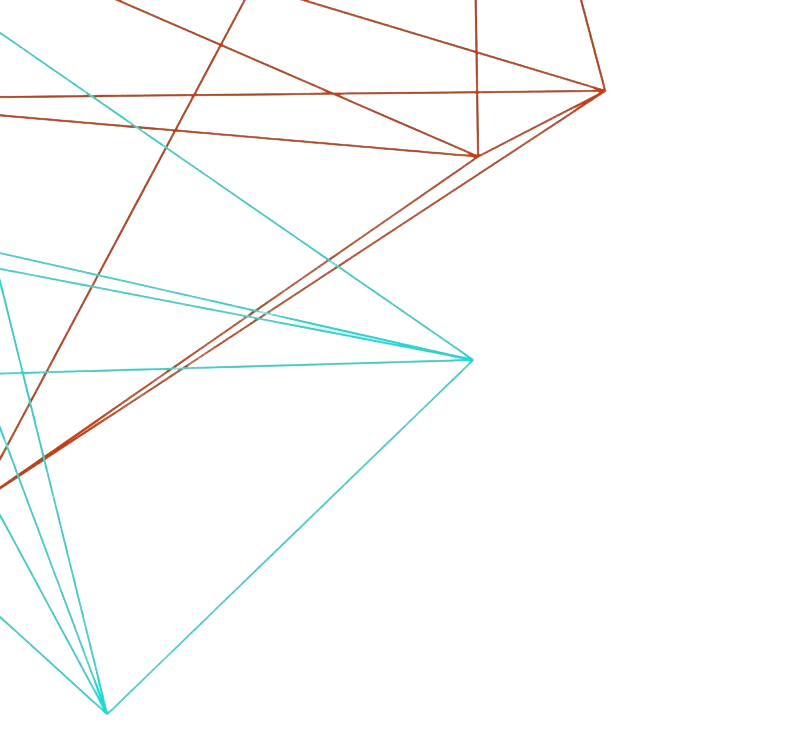
\includegraphics[angle=-90,origin=c,width=0.5\paperheight,height=0.5\paperwidth]{/root/.config/latex-utils/logos/invert3.png}};
\tikz[remember picture,overlay] \node[opacity=0.3,inner sep=0pt, anchor=south east] at (current page.south east){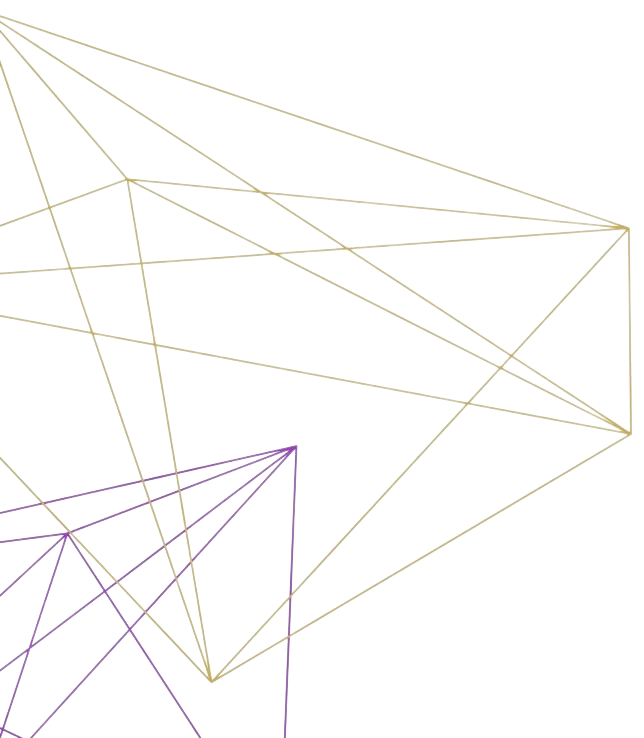
\includegraphics[angle=90,width=0.5\paperwidth,height=0.5\paperheight]{/root/.config/latex-utils/logos/invert2.png}};

\tableofcontents




    
    \newpage

    \section{Contexte et analyse du travail}
     \subsection{Contexte du travail}


      \begin{table}[ht!]
         \centering
         \caption{Tableau de contexte du travail}
         \label{tab:label}
         \begin{tabular}{|l|l|}
            \hline
            \multicolumn{2}{|c|}{\textbf{Identité de l'entreprise}}\\
            \hline
            Intitulé & Laboratoire Hubert-Curien\\
            \hline
            Localisation & Saint-Étienne, Loire, France\\
            \hline
            Secteur d'activité & Recherche et Développement\\
            \hline
            Effectif total & 200\\
            \hline
            \multicolumn{2}{|c|}{\textbf{Tuteur entreprise}}\\
            \hline
            Nom - Prénom & Emmanuel Marin\\
            \hline
            Fonction & Professeur des universités\\
            \hline
         \end{tabular}
     \end{table}


    Le laboratoire Hubert-Curien est un laboratoire de recherche. Il se spécialise, en partie, au capteur à fibres optiques construits à partir de réseaux de Bragg. Ces capteurs sont particulièrement utile pour mesurer des températures, des radiation ou des déformations et peuvent être adaptées pour l'application dans des environments extremes(hautes radiations et hautes températures). 
    
    Ces capteurs peuvent être construit à partir de réseaux de Bragg à pas court(FBG\footnote[1]{Fiber Bragg Gratings}) ainsi que des réseaux de Bragg à pas long(LPG\footnote[2]{Long Period Gratings}). Les FBG ont déjà été étudiés sous condition de températures et radiation élevés c'est donc pour cela que l'on s'intéressera au LPG et les effets sous des condition extrêmes.  
    
    En temps que disposition RSDD, le laboratoire possède un groupe de travail RSE constitué de Mme.Kachan et M.Maselet. Ces derniers s'occupent de résoudre les problématiques de dévelop\-pement durable afin de réduire l'impact environnemental du laboratoire.

    Une partie de son engagement se repose sur les démarches de sécurité mise en place pour les employés. Plusieurs formations sont obligatoires pour l'utilisation de certains équipements scientifiques. Un exemple de ceci est la formation en électronique pour l'utilisation d'équipement spécialisé. Mais ils s'assurent aussi qu'il y ait une sensibilisation envers les danger et risques de ces équipements. Dans mon cas, j'ai du suivre une sensibilisation aux risques lié à l'utilisation de laser femto-seconde. Chaque formation étant suivie par des assistant de prévention pour évaluer les risques et dangers.

    De plus, le laboratoire compartmentalize les zones de travail et d'équipements grâce à des badges d'accès. Chaque badge assurant que les personnes soient autorisées à être dans la zone et que les équipements soient utilisés par des personnes formées. Ceci est notamment important pour des équipements dangerous comme les lasers et les irradiateurs, qui peuvent causer des dommages irréversibles et néfastes pour la santé. 

    Dans le cas des formations liées aux radiations, tout personnel concerné doit participer tout les 3 ans à une formation obligatoire de radioprotection. En plus de cela, ils doivent porter des dosimètres personnels pour mesurer l'exposition aux radiations et ainsi s'assurer que les doses reçues soient en dessous des limites autorisés. Chaque année, un bilan est fait pour évaluer les doses reçues et les risques encourus, suivi par l'agence de sûreté nucléaire(ASN).

    Des tests de santé son également effectués, en particulier pour les opérateurs de lasers, qui sont assujettis à des tests de vision pour s'assurer qu'ils n'ont pas été affectés par des brûlures rétiniennes, qui sont irréversibles et peuvent entraîner une perte de vue partielle ou totale.
    
    
    \subsection{Analyse du travail}

    Mon travail consistait à fabriquer et caractériser des capteurs fait à partir de LPG pour des applications dans des environnements extrêmes. Pour cela il a fallu que je m'informe sur la physique complexe des LPG et des FBG pour comprendre comment ils fonctionnent et les contraintes  de fabrication. Au niveau théorique il a fallu en particulier m'intéresser à la propagation ondulatoire de la lumière dans une fibre, la théorie des modes couplées (et en partie la théorie des perturbations) et la théorie des réseaux de Bragg.

    Une fois ayant compris les bases théoriques, il a fallu que j'effectue une formation obligatoire de sensibilisation aux risques liés à l'utilisation de laser. Cette formation m'a permis de comprendre les dangers liés à l'utilisation de laser femto-seconde et les mesures de sécurité à prendre pour éviter les accidents.
    
    Ce n'est qu'après tout ceci que j'ai pu commencer à travailler sur la partie de la photo-inscription des réseaux de Bragg. Pour me former à cela, j'ai assisté un doctorant dans sa thèse d'inscription de FBG  et le contrôle des spectres d'absorption de ce dernier liée au couplage des modes entre le coeur et la gaine de la fibre, pour des applications permettant une pluri-modalité de mesure (à la fois thermique et deformation physiques). 

    Pendant cette période, nous avions eu des problèmes quand à la qualité du spectre de transmission du FBG. Un problème que l'on pense est lié au caractéristiques du faisceau quand à l'étape de photo-inscription. En considérant le faisceau comme un faisceau gaussien, on hypothèse que la puissance et la taille du faisceau qui touche le coeur dans une zone donné de la fibre modifie donc l'index de réfraction de cette zone à partir de l'effet Kerr optique, et induit par la suite un effet d'autofocalisation du faisceau. 
    Cet effet crée alors sous la zone désirée de photo-inscription des zones de photo-inscription parasites qui dégradent la qualité du spectre de transmission du FBG. 

    Pour tenter de résoudre ce problème nous avons dû revoir la configuration du montage laser, effectuer de nombreux réalignements et ajustements du faisceau afin d'obtenir un faisceau s'approchant le plus possible d'un faisceau gaussien idéal. Il a fallu également revoir les configuration logicielles de la photo-inscription pour s'assurer que les paramètres de photo-inscription soient correctement ajustés, et il a fallu que l'on revoit les condition de génération du faisceau. 

    Chaque composant possédant de nombreux paramètres à ajuster, nous n'avions pas réussi à obtenir des condition de photo-inscription optimales permettant de mitiger ou éliminer les zones parasites.

    La condition de photo-inscription étant un problème majeur, tant pour les FBG que pour les LPG, je n'ai pas encore pu photo-inscrire de LPG. Cependant, j'ai pu observer le processus de photo-inscription et de caractérisation des FBG, ce qui m'a permis de comprendre les étapes de fabrication et de caractérisation des réseaux de Bragg.

     \section{Bilan personnel} 


     Bien que la mission de stage n'aie pas été remplie, j'ai pu acquérir de nombreuses compétences techniques et théoriques. J'ai pu comprendre la physique des réseaux de Bragg et des fibres optiques, et j'ai pu apprendre à manipuler des équipements scientifiques complexes. J'ai également pu apprendre à travailler en équipe et à communiquer avec des personnes de différents horizons, en particulier dans un environment de recherche multilinguistique.

     La fortune d'être trilingue m'a permis de communiquer avec des personnes de différentes nationalités et de comprendre les différentes cultures de travail. J'ai pu également apprendre à travailler de manière autonome et à gérer mon temps de travail de manière efficace. 

     Mes savoir-faire en photonique ont été poussées et améliorés bien au delà de ce que j'aurais pu imaginer. J'ai découvert la rigueur et la précision indispensable à avoir dans un contexte de manipulation de laser ainsi qu'une disposition et une discipline de reflection face au problèmes complexes de la photo-inscription des réseaux de Bragg.

     Grâce à ce stage j'ai pû contraster l'environment de travail en entreprise et en laboratoire. Ceci implique les contraintes de travailler sur un sujet de recherche auparavant non exploré, le ritme de découverte et d'apprentissage lié à la recherche, et la résolution autonome de problèmes apparaissant dans des condition d'experiences uniques. Cela étant bien différent du travail en entreprise, où les problèmes sont souvent déjà résolus et où le travail est plus orienté vers la production et la rentabilité, vis à vis d'un projet définit et déterminé, et d'un respect d'attribution hiérarchique des tâches.

     Ayant adoré le fait d'apprendre tout les jours, je me suis souvent retrouvé à passer plus de temps que prévu au laboratoire ainsi que durant une partie de mon temps libre sur le projet de recherche.

     Dans un contexte de projet professionnel d’ingénieur industriel en photonique, je n'ai jamais entretenu l'idée de la recherche. Ce stage m'as très agréablement surpris et m'as donné une nouvelle perspective sur la recherche en photonique. J'ai pu découvrir un monde de recherche passionnant et enrichissant, ce qui m'encourage désormais à entretenir l'idée de poursuivre une carrière en recherche, ou du moins à forte proximité de la recherche.
     
     Les compétences et les connaissance acquises durant ce stage sont précieuses pour mon projet professionnel, et ont réveillé une passion en photonique que je n'ai que ressenti il y a 5 ans durant un stage sur la caractérisation d'un faisceau gaussien. L'idée et le fait que l'on peut contrôler la lumière pour en faire des applications utiles et innovantes m'as toujours fasciné, et ce stage m'as permis de me rapprocher de cette passion.
     
     
      \begin{table}[ht!]
         \centering
         \caption{Tableau de compétences}
         \label{tab:label}
         \begin{tabular}{|l|c|l|}
        \hline
         \multicolumn{1}{|c}{\textbf{Compétence}} & \multicolumn{1}{|c}{\textbf{Connaisances}} & \multicolumn{1}{|c|}{\textbf{Application}} \\
        \hline
        \multirow{3}{*}{\textbf{Photonique}} & \multirow{3}{*}{\begin{tabular}[c]{@{}c@{}}Propagation ondulatoire de la lumière\\ Modes couplés\\ Réseaux de Bragg\end{tabular}} & \multirow{3}{*}{\begin{tabular}[c]{@{}l@{}} Charactérisation et simulation\\ du couplage et propagation\\ de la lumière \end{tabular}} \\
         & & \\
         & & \\
        \hline 
        \multirow{3}{*}{\textbf{Sécurité}} & \multirow{3}{*}{\begin{tabular}[c]{@{}c@{}}Sensibilisation aux risques\\ liés à l'utilisation de laser\\ Formation en radioprotection\end{tabular}} & \multirow{3}{*}{\begin{tabular}[c]{@{}l@{}}Application des règles de sécurité\\ lors de l'utilisation de laser\\ et de radiations\end{tabular}} \\
            & & \\
            & & \\
        \hline
        \multirow{3}{*}{\textbf{Travail en équipe}} & \multirow{3}{*}{\begin{tabular}[c]{@{}c@{}}Communication interculturelle\\ Travail en équipe\\ Gestion du temps\end{tabular}} & \multirow{3}{*}{\begin{tabular}[c]{@{}l@{}} Resolution de problèmes\\
        Apports de connaissance et aide\\ \end{tabular}} \\
            & & \\
            & & \\
        \hline 
        \multirow{2}{*}{\textbf{Autonomie}} & \multirow{2}{*}{\begin{tabular}[c]{@{}c@{}}Travail autonome\\ Rigueur et précision\end{tabular}} & \multirow{2}{*}{\begin{tabular}[c]{@{}l@{}}Recherche \\ Résolution de problèmes\end{tabular}} \\
            & & \\
        \hline
         \end{tabular}
     \end{table}


\end{document}